\documentclass[%
	%draft,
	%submission,
	%compressed,
	final,
	%
	%technote,
	%internal,
	%submitted,
	%inpress,
	%reprint,
	%
	%titlepage,
	notitlepage,
	%anonymous,
	narroweqnarray,
	inline,
	%twoside,
        %invited,
	]{ieee}
\usepackage{graphicx}
\usepackage{hyperref}
\usepackage{listings}
\lstset{
  language=R,
  basicstyle=\scriptsize\ttfamily,
  commentstyle=\ttfamily\color{gray},
  numbers=left,
  numberstyle=\ttfamily\color{gray}\footnotesize,
  stepnumber=1,
  numbersep=5pt,
  backgroundcolor=\color{white},
  showspaces=false,
  showstringspaces=false,
  showtabs=false,
  frame=single,
  tabsize=2,
  captionpos=b,
  breaklines=true,
  breakatwhitespace=false,
  title=\lstname,
  escapeinside={},
  keywordstyle={},
  morekeywords={}
}


\lstloadlanguages{R}
\newcommand{\latexiie}{\LaTeX2{\Large$_\varepsilon$}}
\begin{document}

\nocite{big}
\nocite{Sh:1}
\nocite{small} 

\title[Topic Networks]{
       Topic Networks \\
       {\Large A mini project for Social Network Analysis}
}
%\author[Bob Flagg]{Bob Flagg}

%\firstpage{}


\maketitle               
% ---------------------------------------------------------------------------- %
% Introduction                                                                 %
% ---------------------------------------------------------------------------- %
\section{Introduction}

\PARstart Automatic text summarization is a challenging problem whose solution 
would allow users to browse large document collections and quickly view highlights 
and drill down for details.  
%would provide a valuable tool in dealing with the {\it information explosion} 
%by allowing users to browse large document collections and quickly view highlights 
%and drill down for details.  
In this project we attempt to bring the power of social network analysis to bear on
this problem by developing 
a new approach to summarizing document collections, using topic models and bipartite 
graphs. 

Our method first builds a topic model for a document collection using 
\href{http://en.wikipedia.org/wiki/Latent_Dirichlet_allocation}{Latent Dirichlet allocation}\cite{lda}.
This topic model naturally defines a \href{http://en.wikipedia.org/wiki/Bipartite_graph}{bipartite graph}\cite{bipartite} 
between documents and the topics that appear in 
them.  The bipartite graph is converted into a network of topics by linking
topics if they appear in the same document.  By analyzing a simple sample corpus, we explore 
properties of these {\em topic networks} in hopes that they will
provide insights useful in summarizing the
underlying document collection.


\section{A Simple Example}

\PARstart To demonstrate topic networks we will use a simple example consisting of
texts of 102 speeches given by Barack Obama prior to his 2009 Inauguration scraped from 
\href{http://obamaspeeches.com/}{obamaspeeches.com}\cite{speeches} on April 12, 2013.
We'll use the {\bf R} programming language\cite{cran} for this demo. All the steps
are reproduced below and in an R source file available on
\href{https://github.com/bobflagg/Topic-Networks}{GitHub}\cite{github}. We have
borrowed a lot of ideas from Solomon Messing's blog post\cite{messing} on 
working with bipartitie/affiliation networks in {\bf R}.

\subsection{The Document-Term Matrix}

\PARstart If the path to the directory containing the texts of Obama speeches is in
the variable {\tt corpus.source}, then we can build the corpus and document-term matrix
with the following commands:

\begin{verbatim}

# Load the text mining package
require(tm, quietly=TRUE)
# Build the corpus.
corpus.source <- DirSource(corpus.directory, 
  encoding="UTF-8")
corpus <- Corpus(corpus.source)
corpus.copy <-corpus
# Build the document term matrix.
corpus.dtm <- DocumentTermMatrix(
  corpus, 
  control = list(
    stemming = TRUE, 
    stopwords = TRUE, 
    minWordLength = 3,
    removeNumbers = TRUE, 
    removePunctuation = TRUE
  )
)
\end{verbatim}

\subsection{Frequent Words}

\PARstart To gain some preliminary insight into this corpus, we'll 
look at a bar chart of most frequent words and a word cloud.

\begin{verbatim}

# Load required packages:
require(RColorBrewer, quietly=TRUE)
# Sort terms by frequency:
word.freq <- sort(col_sums(corpus.dtm), 
  decreasing=TRUE)
# barplot with the top 20 most frequent terms
top.terms <- head(word.freq, n=20)
# complete the stems and fix missing values and errors:
completions <- stemCompletion(names(top.terms), 
  dictionary=corpus.copy, type="prevalent")
completions<-ifelse(completions == "", names(top.terms), 
  completions)
names(top.terms) <-completions
names(top.terms)[10] <-"every"
pdf("mostfreq.pdf")
op <- par(mar = c(4,6.1,.1,.2))
barplot(top.terms, las=2, horiz=TRUE)
dev.off()
# wordcloud
pal2 <- brewer.pal(8,"Dark2")
top.terms <- head(word.freq, n=1200)
completions <- stemCompletion(names(top.terms), 
  dictionary=corpus.copy, type="prevalent")
completions<-ifelse(completions == "", names(top.terms), 
  completions)
names(top.terms) <-completions
pdf("wordcloud.pdf")
par(mar = c(0,0,0,0))
wordcloud(
  words=names(top.terms), 
  freq=top.terms, 
  min.freq=20, 
  random.order=F, 
  colors=pal2, 
  rot.per=.15
)
dev.off()
\end{verbatim}

\begin{figure}[ht!]
\centering
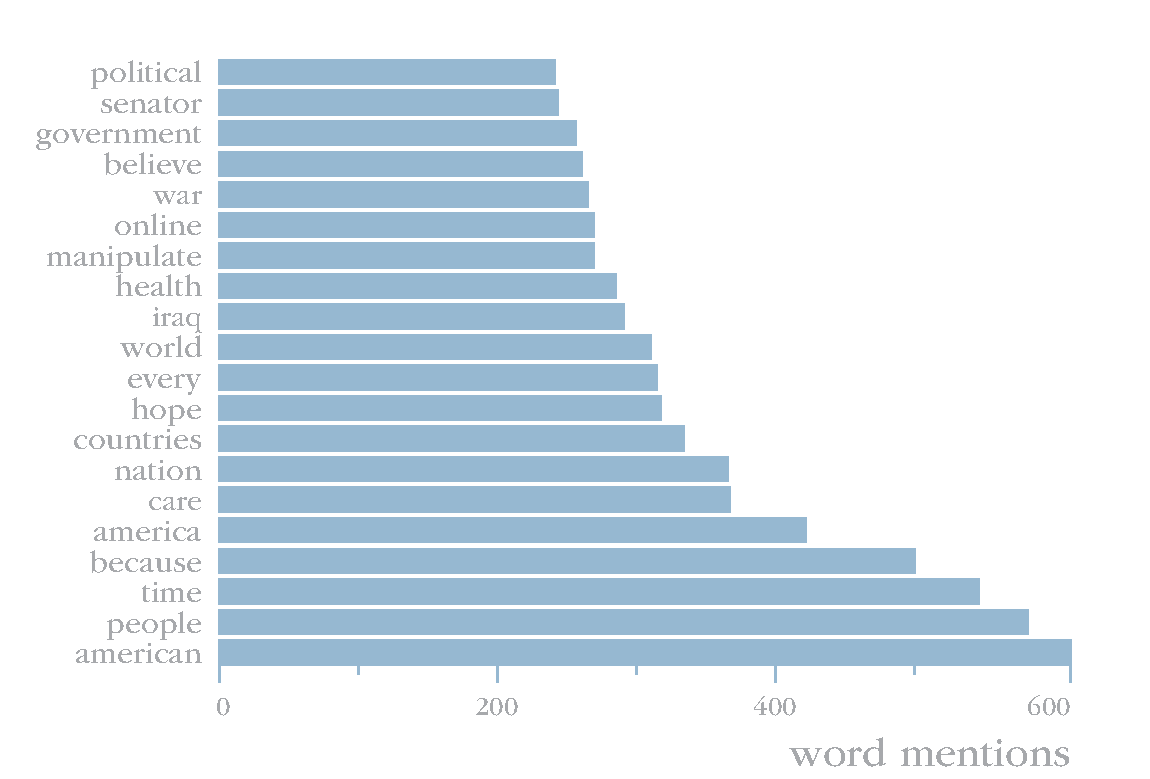
\includegraphics[width=90mm]{mostfreq.pdf}
\caption{Most frequent words}
\label{fig:barchart}
\end{figure}

\begin{figure}[ht!]
\centering
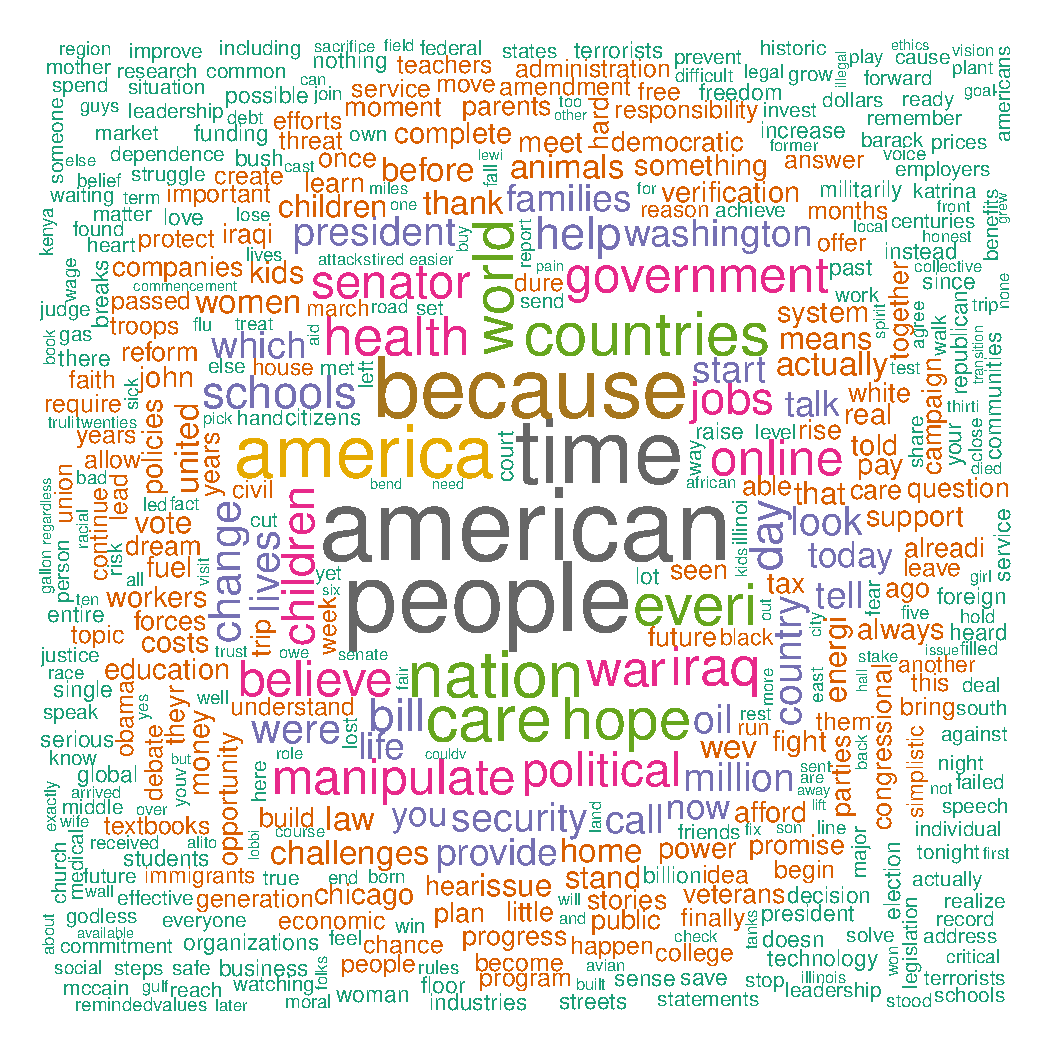
\includegraphics[width=90mm]{wordcloud.pdf}
\caption{Wordcloud: frequency $\geq$ 20}
\label{fig:wordcloud}
\end{figure}

\subsection{The Topic Model}

\PARstart Before building a topic model, we want to filter out ``unimportant'' words from
the corpus. For this we will use the tf-idf matrix.

\begin{verbatim}
# Build the tf-idf matrix:
term.tfidf <- tapply(
 corpus.dtm$v/row_sums(corpus.dtm)[corpus.dtm$i], 
 corpus.dtm$j, mean) * 
 log2(nDocs(corpus.dtm)/col_sums(corpus.dtm > 0))
# Filter out "unimportant" terms:
dtm <- corpus.dtm[,term.tfidf >= 0.01]
dtm <- dtm[row_sums(dtm) > 0,]
\end{verbatim}

Now we build the topic model and collect collect relevant data in a data frame.

\begin{verbatim}
require(topicmodels, quietly=TRUE)
# Build a topic model:
corpus.tm <- LDA(dtm, k = 22)
corpus.tm.terms <- terms(corpus.tm, 3)
corpus.tm.topics <- topics(corpus.tm, 4)
topic.labels <- apply(corpus.tm.terms, 2, 
  function(x) paste(x, collapse=", "))
document.labels <- colnames(corpus.tm.topics)
dt.df <- data.frame(
  document=rep(document.labels, each=4),
  topic=as.vector(corpus.tm.topics)
)
# Replace doucment labels with numbers:
dt.df$document <- as.numeric(gsub(".txt","",
  dt.df$document))
# Order the data according to document number:
dt.df <- dt.df[order(dt.df$document),]
\end{verbatim}


\subsection{The Document-Topic Network}
\PARstart The first network we'll consider has two modes: documents and topics. 
The {\tt igraph} package allows us to construct a network from an incidence 
matrix as follows.

\begin{verbatim}
require(igraph, quietly=TRUE)
# Build the incidence matrix:
dt.matrix <- as.matrix(table(dt.df))
# Build the document-topic network:
dt.network <- graph.incidence(dt.matrix)


corpus.tm <- LDA(dtm, k = 22)
corpus.tm.terms <- terms(corpus.tm, 3)
corpus.tm.topics <- topics(corpus.tm, 4)
topic.labels <- apply(corpus.tm.terms, 2, 
  function(x) paste(x, collapse=", "))
document.labels <- colnames(corpus.tm.topics)
dt.df <- data.frame(
  document=rep(document.labels, each=4),
  topic=as.vector(corpus.tm.topics)
)
# Replace doucment labels with numbers:
dt.df$document <- as.numeric(gsub(".txt","",
  dt.df$document))
# Order the data according to document number:
dt.df <- dt.df[order(dt.df$document),]
\end{verbatim}

Figure \ref{fig:dtn}, which was generated with the code below, 
shows the document-topic network, with 
topic nodes displayed as large green dots to distinquish them from
document nodes.


\begin{verbatim}
n.docs <- nrow(dt.matrix)
n.topics <- ncol(dt.matrix)
n.vertices <- n.docs + n.topics
V(dt.network)$color[1:n.docs] <- 
  rgb(1,0,0,.4)
V(dt.network)$color[(n.docs+1):n.vertices] <- 
  rgb(0,1,0,.5)
V(dt.network)$label <- NA
V(dt.network)$size[1:n.docs] <- 2
V(dt.network)$size[(n.docs+1):n.vertices] <- 6
E(dt.network)$width <- .5
E(dt.network)$color <- rgb(.5,.5,0,.4)
pdf("dtn.pdf")
plot(dt.network, 
  layout=layout.fruchterman.reingold)
dev.off()
\end{verbatim}


\begin{figure}
\centering
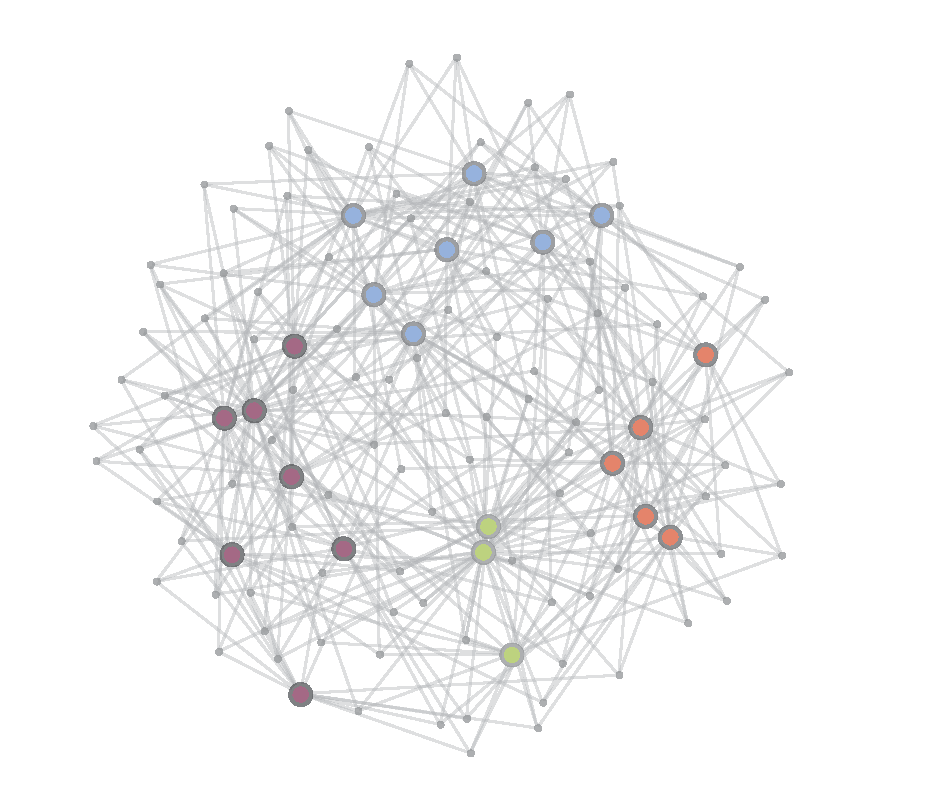
\includegraphics[width=90mm]{dtn.pdf}
\caption{Document-Topic Network}
\label{fig:dtn}
\end{figure}


\subsection{The Topic Network}

\PARstart The topic network is the one of most interest to us.  To build it
we create its adjacency matrix by multiplying the transpose of the document-topic
matrix with itself.

\begin{verbatim}
# Create the topic network:
topic.network.matrix <- t(dt.matrix) %*% dt.matrix
topic.network <- graph.adjacency(
  topic.network.matrix, mode = "undirected")
\end{verbatim}

Figure \ref{fig:topic-network}, which was created with the code below, shows the 
topic network, with 
topic nodes labelled by the three most probable terms in the corresponding
topic distribution.

\begin{verbatim}
E(topic.network)$weight <- 
  count.multiple(topic.network)
topic.network <- simplify(topic.network)
# Set vertex attributes
V(topic.network)$label <- topic.labels
V(topic.network)$label.color <- rgb(0,0,0,1)
V(topic.network)$label.cex <- .75
V(topic.network)$size <- 8
V(topic.network)$color <- rgb(0,1,0,.6)
# Set edge gamma according to edge weight
egam <- (log(E(topic.network)$weight)+.3)/
  max(log(E(topic.network)$weight)+.3)
E(topic.network)$color <- rgb(.5,.5,0,egam)
pdf("topic-network.pdf")
plot(topic.network, layout=layout.kamada.kawai)
dev.off()
\end{verbatim}


\begin{figure}
\centering
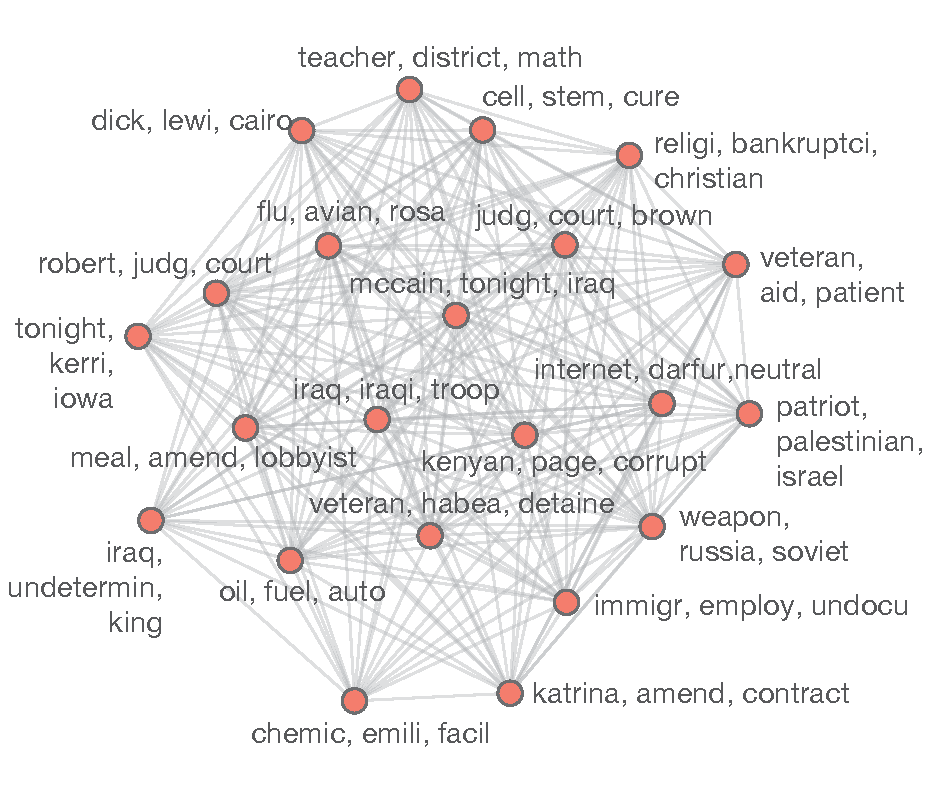
\includegraphics[width=90mm]{topic-network.pdf}
\caption{Topic Network}
\label{fig:topic-network}
\end{figure}



\subsection{The Overlap Network}

\PARstart Another interesting view of this data takes into account the 
percent overlap between topics, which gives rise to a directed network.
To create this graph, we divide each row by the diagonal to get the
adjacency matrix.

\begin{verbatim}
overlap.matrix <- topic.network.matrix / 
  diag(topic.network.matrix)
overlap.network <- graph.adjacency(
  overlap.matrix, weighted=T)
\end{verbatim}

We use the density plot show in Figure~\ref{fig:density} to choose
a reasonable cut-off value for removing some noise in the edges before plotting this
network.  

\begin{verbatim}
pdf("density.pdf")
plot(density(overlap.matrix), main=NA, xlab=NA)
dev.off()
overlap.matrix[overlap.matrix < 0.2] <- 0
overlap.network <- graph.adjacency(overlap.matrix, 
  weighted=T)
overlap.network <- simplify(overlap.network, 
  remove.multiple=FALSE, remove.loops=TRUE)
overlap.network$layout <- layout.kamada.kawai(
  overlap.network)
V(overlap.network)$label <- topic.labels
tkplot(overlap.network)
overlap.network$layout <- tkplot.getcoords(1)
\end{verbatim}


The final step to display this network in a way to make the
important properties visable requires some manual work.  We'll use the
tkplot gui tool to help us layout nodes so that labels are clearly
visible. Once we're done arranging nodes, the layout can be saved
using {\tt tkplot.getcoords(1)}:


\begin{verbatim}
overlap.network$layout <- layout.kamada.kawai(
  overlap.network)
V(overlap.network)$label <- topic.labels
tkplot(overlap.network)
overlap.network$layout <- tkplot.getcoords(1)
\end{verbatim}

\noindent Finally, we set a number of properties to improve the
visualization:


\begin{verbatim}
V(overlap.network)$label.color <- rgb(0,0,.2,.6)
V(overlap.network)$label.cex <- .75
V(overlap.network)$size <- 6
#V(topic.network)$frame.color <- NA
V(overlap.network)$color <- rgb(0,1,0,.6)

# Set edge gamma according to edge weight
egam <- (E(overlap.network)$weight+.1)/max(
  E(overlap.network)$weight+.1)
E(overlap.network)$color <- rgb(.5,.5,0,egam)
E(overlap.network)$arrow.size <- .3
V(overlap.network)$label.cex <- 
  degree(overlap.network)/(max(degree(
    overlap.network)/2))+ .3
pdf("overlap-network.pdf")
plot(overlap.network)
dev.off()
\end{verbatim}

\begin{figure}
\centering
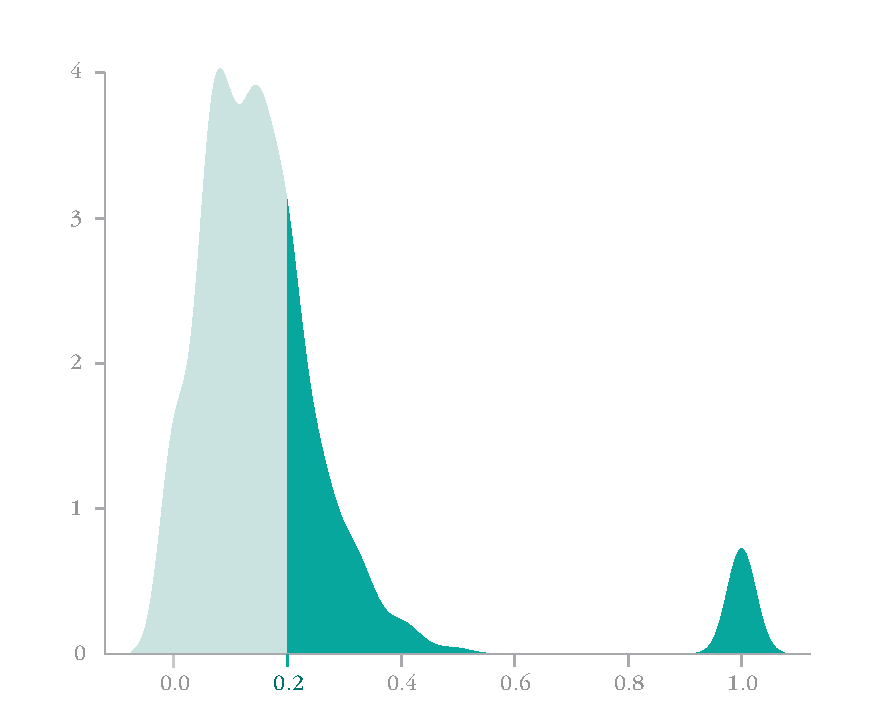
\includegraphics[width=90mm]{density.pdf}
\caption{Density Plot}
\label{fig:density}
\end{figure}

\noindent Figure~\ref{fig:overlap-network} shows the results.

\begin{figure}
\centering
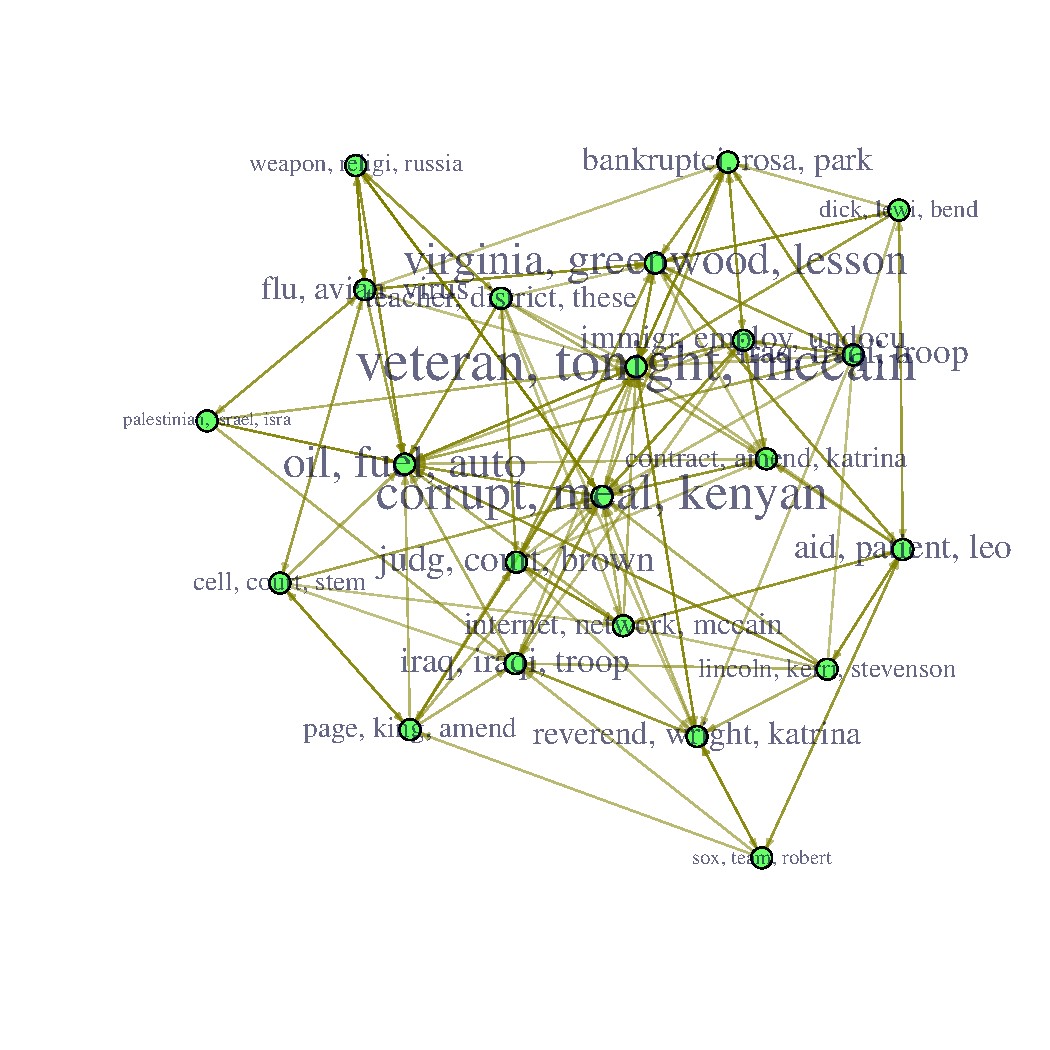
\includegraphics[width=90mm]{overlap-network.pdf}
\caption{Topic Overlap Network}
\label{fig:overlap-network}
\end{figure}



%%
% ---------------------------------------------------------------------------- %
% Conclusions                                                                  %
% ---------------------------------------------------------------------------- %
\section{Conclusions}

\PARstart Our simple example suggests that topic networks may be useful in analyzing 
document collections.  However, we have only scratched the surface
here and much more work is required to confirm this hypothesis as well as to investigate
properties of topic networks and applications to document collection summarization.

\begin{thebibliography}{1}

\bibitem{bipartite}
From Wikipedia, the free encyclopedia \\
\newblock {\em Bipartite graph}, \\
\newblock \url{http://en.wikipedia.org/wiki/Bipartite_graph}

\bibitem{github}
Topic Networks GitHub repository \\
\newblock \url{https://github.com/bobflagg/Topic-Networks}

\bibitem{lda}
From Wikipedia, the free encyclopedia \\
\newblock {\em Latent Dirichlet allocation}, \\
\newblock \url{http://en.wikipedia.org/wiki/Latent_Dirichlet_allocation}

\bibitem{messing}
Solomon Messing, \\
\newblock {\em Working with Bipartite/Affiliation Network Data in R}, \\
\newblock \url{http://solomonmessing.wordpress.com/2012/09/30/working-with-bipartiteaffiliation-network-data-in-r/}

\bibitem{speeches}
Best Speeches of Barack Obama through his 2009 Inauguration \\
\newblock \url{http://obamaspeeches.com/}


\bibitem{cran}
R Core Team (2012),
\newblock {\em R: A language and environment for statistical computing.},
\newblock \url{http://www.R-project.org}

\bibitem{smartlab}
Jorge L. Reyes-Ortiz, Davide Anguita, Alessandro Ghio, Luca Oneto,
\newblock {\em Human Activity Recognition Using Smartphones Dataset.},
\newblock Smartlab - Non Linear Complex Systems Laboratory

\bibitem{r-markdown}
R Core Team (2012),
\newblock {\em R Markdown},
\newblock \url{http://www.rstudio.com/ide/docs/authoring/using_markdown}
\newblock Accessed 2/12/2013

\bibitem{elemstatlearn}
Trevor Hastie, Robert Tibshirani, Jerome Friedman
\newblock {\em The Elements of Statistical Learning},
\newblock Springer, 2011.


\end{thebibliography}

\end{document}




In particular, we compute the degree distribution
and investigate centrality, path length and community structure.

Below we demonstrate topic networks on a small corpora of 

Source code for our work is available at ...
% ---------------------------------------------------------------------------- %
% Methods                                                                      %
% ---------------------------------------------------------------------------- %

\begin{verbatim}
# Build the document term matrix.
corpus.dtm <- DocumentTermMatrix(
  corpus, 
  control = list(
    stemming = TRUE, 
    stopwords = TRUE, 
    minWordLength = 3,
    removeNumbers = TRUE, 
    removePunctuation = TRUE
  )
)
\end{verbatim}
